\documentclass[border=4pt]{standalone}
\usepackage{tikz}
\usetikzlibrary{arrows.meta,positioning,fit,calc,backgrounds}
\usepackage[T1]{fontenc}
\usepackage{lmodern}
\usepackage{amsmath,amssymb}
\definecolor{wsp}{HTML}{2A78D6}
\definecolor{dflt}{HTML}{7A7974}
\definecolor{trn}{HTML}{EB6834}
\definecolor{sb}{HTML}{1BAF7A}
\definecolor{look}{HTML}{6250D6}
\definecolor{ink}{HTML}{0B0B0B}
\definecolor{ink2}{HTML}{52514E}
\definecolor{paper}{HTML}{F4F3EF}
\tikzset{
  box/.style={draw=ink2, rounded corners=3pt, fill=paper, align=center, inner sep=5pt, font=\small, text width=#1},
  box/.default=3.0cm,
  hl/.style={draw=wsp, line width=0.9pt, fill=wsp!8},
  arr/.style={-{Stealth[length=2.2mm]}, line width=0.7pt, draw=ink2},
  note/.style={font=\footnotesize\itshape, text=ink2, align=center},
}

\begin{document}
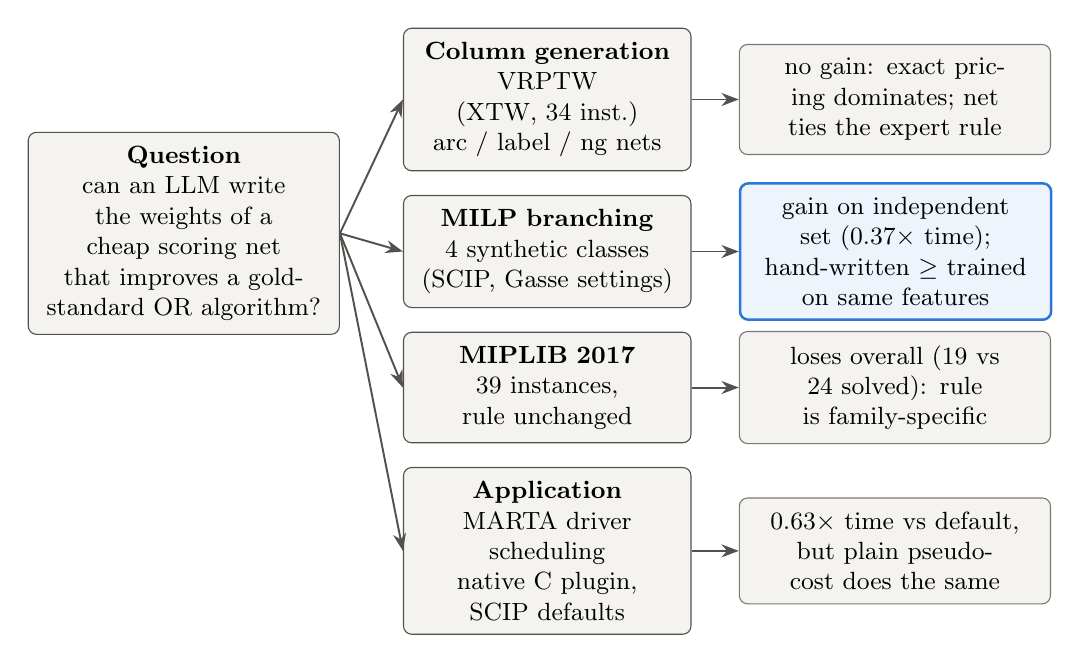
\begin{tikzpicture}[node distance=3mm and 4mm]
\node[box=3.6cm] (q) {\textbf{Question}\\ can an LLM write the weights of a cheap scoring net that improves a gold-standard OR algorithm?};
\node[box=3.3cm, right=8mm of q, yshift=17mm] (cg) {\textbf{Column generation}\\ VRPTW (XTW, 34 inst.)\\ arc / label / ng nets};
\node[box=3.3cm, below=of cg] (syn) {\textbf{MILP branching}\\ 4 synthetic classes\\ (SCIP, Gasse settings)};
\node[box=3.3cm, below=of syn] (mip) {\textbf{MIPLIB 2017}\\ 39 instances, rule unchanged};
\node[box=3.3cm, below=of mip] (marta) {\textbf{Application}\\ MARTA driver scheduling\\ native C plugin, SCIP defaults};
\node[box=3.6cm, right=6mm of cg, draw=dflt] (v1) {no gain: exact pricing dominates; net ties the expert rule};
\node[box=3.6cm, right=6mm of syn, hl] (v2) {gain on independent set (0.37$\times$ time); hand-written $\geq$ trained on same features};
\node[box=3.6cm, right=6mm of mip, draw=dflt] (v3) {loses overall (19 vs 24 solved): rule is family-specific};
\node[box=3.6cm, right=6mm of marta, draw=dflt] (v4) {0.63$\times$ time vs default, but plain pseudocost does the same};
\foreach \n in {cg,syn,mip,marta}{\draw[arr] (q.east) -- (\n.west);}
\draw[arr] (cg)--(v1); \draw[arr] (syn)--(v2); \draw[arr] (mip)--(v3); \draw[arr] (marta)--(v4);
\end{tikzpicture}
\end{document}
